\section{Vorbereitung}

\subsection{Aufgabe V1.1}

% Rekapitulieren Sie die Begriffe Kennlinienfeld, Arbeitspunkt und stationäres Verhalten. Welche Gleichung im Grundlagenteil beschreibt die zu messenden Kennlinienfelder und welche (mathematischen) Abhängigkeiten erwarten Sie für uyϑ = f(uuP ) bzw. uyϑ = f(uuL)?

\subsubsection{Kennlinienfeld}

Ein Kennlinienfeld ist eine Darstellung von mehreren Kennlinien von einem System im gleichen Diagramm, die sich um einen Parameter unterscheiden.

\subsubsection{Arbeitspunkt}

Der Arbeitspunkt ist ein Punkt auf der Kennlinie, an dem der Zustand eines Systems im Betrieb gehalten wird.

\subsubsection{Stationäres Verhalten}

Ein System zeigt sein stationäres Verhalten, wenn äußere Einflüsse sich nicht verändern und das System eingeschwungen ist.

\subsubsection{Gleichung der Kennlinienfelder}

Die für uns interessanten Kennlinien beschreiben den Temperaturanstieg in Abhängigkeit von der zugeführten Leistung. Weitere Parameter sind die die Dichte und spezifische Wärmekapazität der Luft, sowie die Strömungsgeschwindigkeit. 

\[ \Delta\vartheta  = \frac{1}{c_L \varrho_L A}\frac{1}{v}P_{th} \]

Durch erhöhen der Strömungsgeschwindigkeit wird die Temperatur abfallen, da die zugeführte Energie auf mehr Luftmasse aufgeteilt wird. Durch erhöhen der Heizleistung erhöht sich die Temperatur, da die Luft eine höhere Energiemenge aufnehmen muss.

\subsection{Aufgabe V1.2}

% Berechnen Sie mit Hilfe der Übertragungsfunktion einen analytischen Ausdruck für die Sprungantwort des Temperaturverlaufs bei einem Heizleistungssprung Pel(t) = Pˆelσ(t).

\[ G_{S}(s) = \frac{\vartheta(s)}{P_{el}(s)} = K_{S} \frac{e^{-T_{t}s}}{1 + T_{S}s} \]
\[ \]


\[ \vartheta\left(t\right) = \hat{P}_{el} \cdot K_s \cdot \left(1-e^{-\frac{1}{T_s}\cdot\left(t-T_t\right) }\right) \]

\subsection{Aufgabe V1.3 und Aufgabe V1.4}

% Simulieren und plotten Sie den Zeitverlauf der Sprungantwort mit Matlab/Simulink für Pel(t) = 10 W · σ(t).

% Rekapitulieren Sie aus dem Grundlagenteil den Einfluss (mathematische Abhängigkeit) der Heizleistung auf die Streckenparameter. Plotten oder skizzieren Sie hierzu die Sprungantworten für a) Pel(t) = 10 W · σ(t), b) Pel(t) = 20 W · σ(t), c) Pel(t) = 30 W · σ(t). und überlegen Sie sich eine physikalische Interpretation.

In \autoref{fig:V1_4_kennlinienfeld} wird das Kennlinienfeld für \( P_{el} = \SI{10}{\watt}\), \(\SI{20}{\watt}\) und \(\SI{30}{\watt}\) gezeigt. Es ist deutlich zu erkennen, dass eine höhere zugeführte Leistung mit einer höheren Temperaturänderung einhergeht. Das liegt daran, dass eine höhere Leistung dem System im gleichen Zeitraum eine größere thermische Energiemenge zuführt. Dadurch muss auch die Temperatur stärker ansteigen.

\begin{figure}[H]
    \begin{center}
        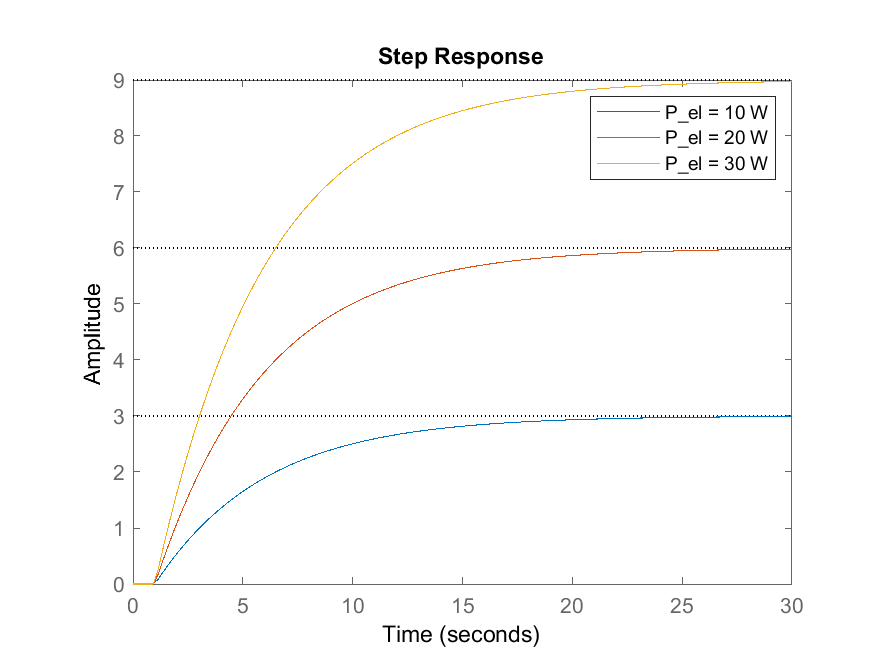
\includegraphics[width=0.8\textwidth]{img/V1_4.png}
        \caption{Kennliniefeld für \( P_{el} = \SI{10}{\watt}\), \(\SI{20}{\watt}\) und \(\SI{30}{\watt}\)}
        \label{fig:V1_4_kennlinienfeld}
    \end{center}
\end{figure}

\newpage

\subsection{Aufgabe V1.5}

% Wiederholen Sie V1.4 mit dem Einfluss der Lüftergeschwindigkeit und überlegen Sie sich, was passiert, wenn man die Lüftergeschwindigkeit halbiert bzw. verdoppelt. Plotten oder skizzieren Sie hierzu die Temperaturverläufe für Pel(t) = 10 W · σ(t) unter der Annahme der folgenden Strömungsgeschwindigkeiten: a) v = vL, b) v = vL 2 , c) v = 2 · vL.

In \autoref{fig:V1_5_kennlinienfeld} wird das Kennlinienfeld für \( v = v_L\), \(\frac{v_L}{2}\) und \(2\cdot v_L\) gezeigt. Die erreichte Temperaturänderung halbiert sich bei doppelter Strömungsgeschwindigkeit und verdoppelt sich bei halbierung der Strömungsgeschwindigkeit. Das liegt daran, dass sich die dem System zugeführte Energie im gleichen Zeitraum auf die halbe bzw. doppelte Menge Luft kommt.

\begin{figure}[H]
    \begin{center}
        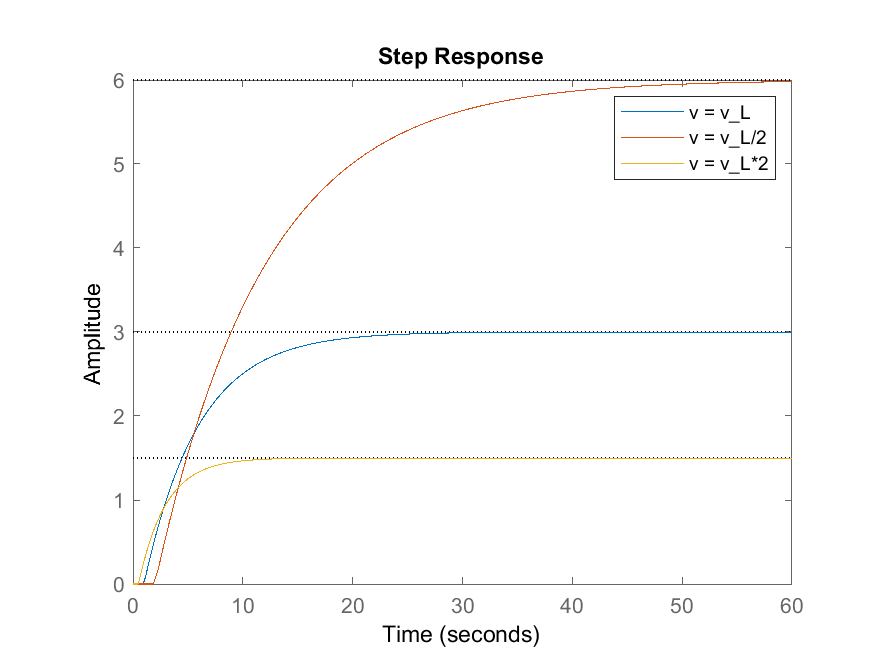
\includegraphics[width=0.8\textwidth]{img/V1_5.png}
        \caption{Kennliniefeld für \( v = v_L\), \(\frac{v_L}{2}\) und \(2\cdot v_L\)}
        \label{fig:V1_5_kennlinienfeld}
    \end{center}
\end{figure}

\newpage